\begin{figure}[h!]
  \begin{center}
    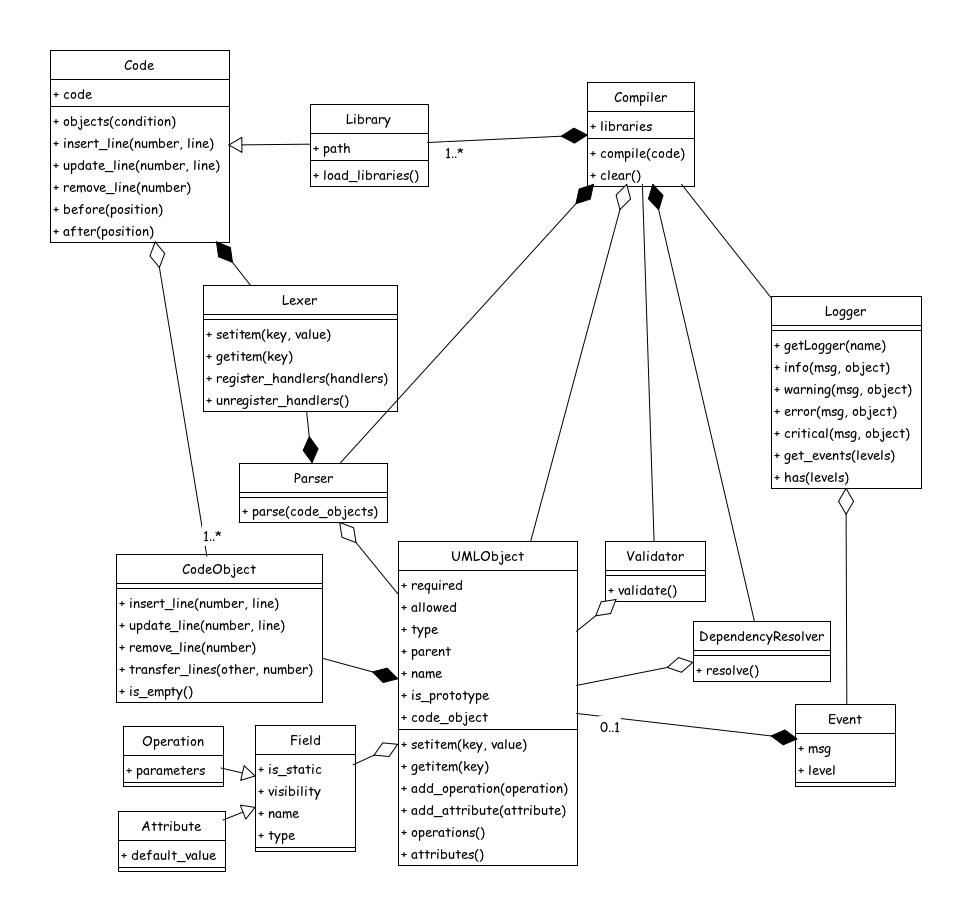
\includegraphics[width=\textwidth]{compiler}
  \end{center}
  \caption{Diagram klas modułu \texttt{compiler}}
\end{figure}

\begin{figure}[h!]
  \begin{center}
    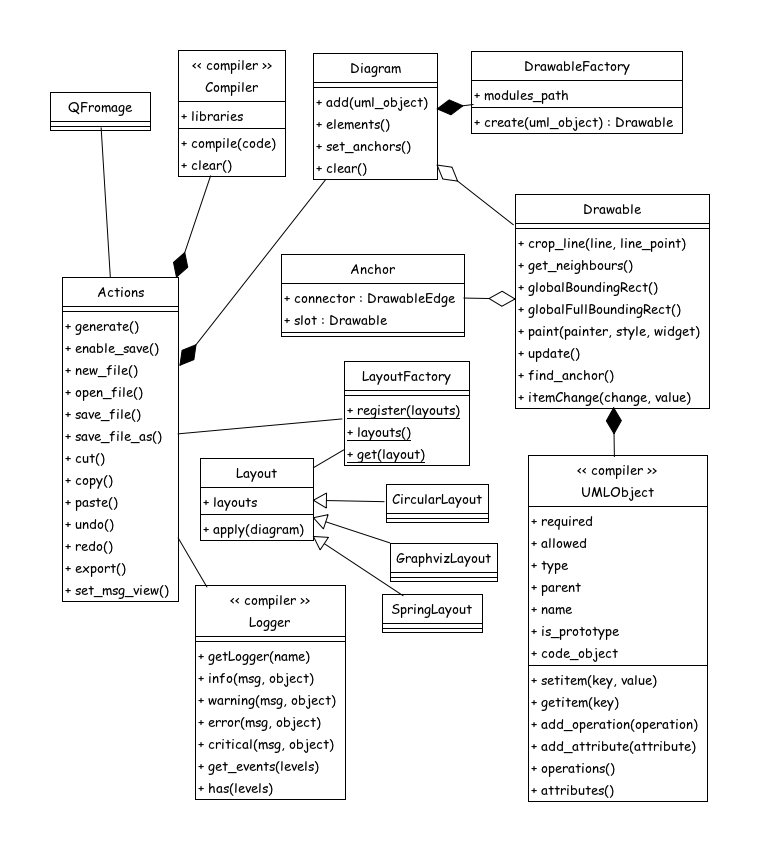
\includegraphics[width=\textwidth]{fromage}
  \end{center}
  \caption{Diagram klas modułu \texttt{fromage}}
\end{figure}

\begin{figure}[h!]
  \begin{center}
    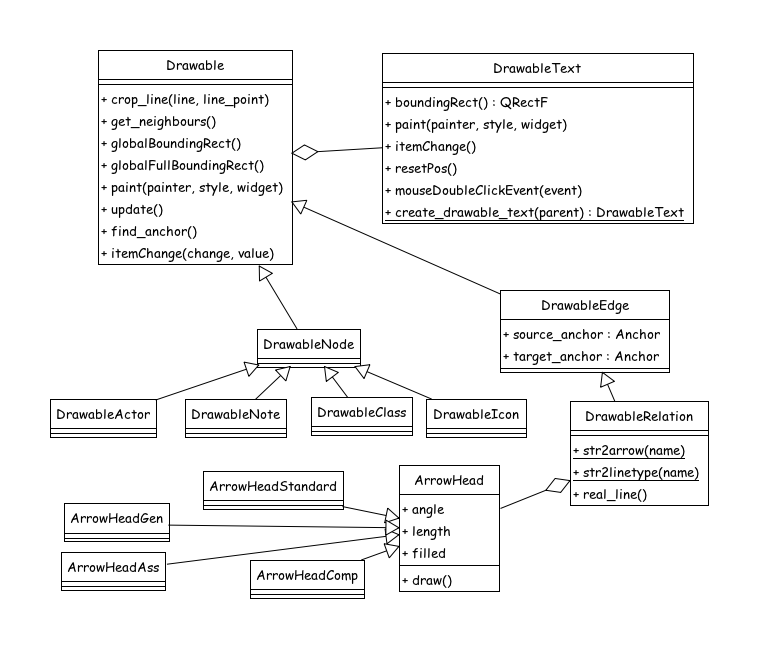
\includegraphics[width=\textwidth]{drawable}
  \end{center}
  \caption{Diagram klas modułu \texttt{modules}}
\end{figure}
